\documentclass[10pt]{article}
\usepackage[english]{babel}
\usepackage{../../../meta-inf/lib/naproche}
\usepackage{amssymb}
\usepackage{mathtools} % for \coloneq

\usepackage{stex-highlighting}
\providebool{emph} % "\newbool{emph}" does not work...
\setbool{emph}{false}
\colorlet{emphcolor}{violet}
\let\oldemph\emph
\renewcommand\emph[1]{\setbool{emph}{true}\ifbool{forthel}{\textcolor{emphcolor}{\itshape#1}}{\oldemph{#1}}\setbool{emph}{false}}
\renewcommand{\varemph}[1]{\ifbool{emph}{\textcolor{emphcolor}{#1}}{\textcolor{black}{#1}}}

\usepackage[right=6cm,left=3cm,bottom=3cm,marginparwidth=5cm]{geometry}

\usepackage{fancyhdr}
\renewcommand{\sectionmark}[1]{\markboth{#1}{}} 
\def\libarchive{}
\pagestyle{fancy}
\fancyhead[L]{\libarchive}
\fancyhead[C]{\nouppercase\leftmark}  % section title
\fancyhead[R]{\thepage}               % page number
\fancyfoot[C]{}                       % No page number in footer

\usepackage[nobottomtitles]{titlesec}
\titlespacing*{\section}{0pt}{30pt}{0pt}
\titlespacing*{\subsection}{0pt}{30pt}{0pt}
\titlespacing*{\subsubsection}{0pt}{30pt}{0pt}

\documentclass[12pt,oneside]{book}

\usepackage[foundations]{../../lib/tex/naproche}
\usepackage{../../lib/tex/libraries}
\usepackage{graphicx}
\usepackage{float}
\usepackage{caption}
\usepackage{footnote}

\makesavenoteenv{tabular} % Make footnotes work in tabular environments


\title{Foundations of Mathematics}
\author{Marcel Schütz}
\date{2022}

\begin{document}
  \maketitle

  \tableofcontents

  \begin{figure}[H]
    \centering
    \fbox{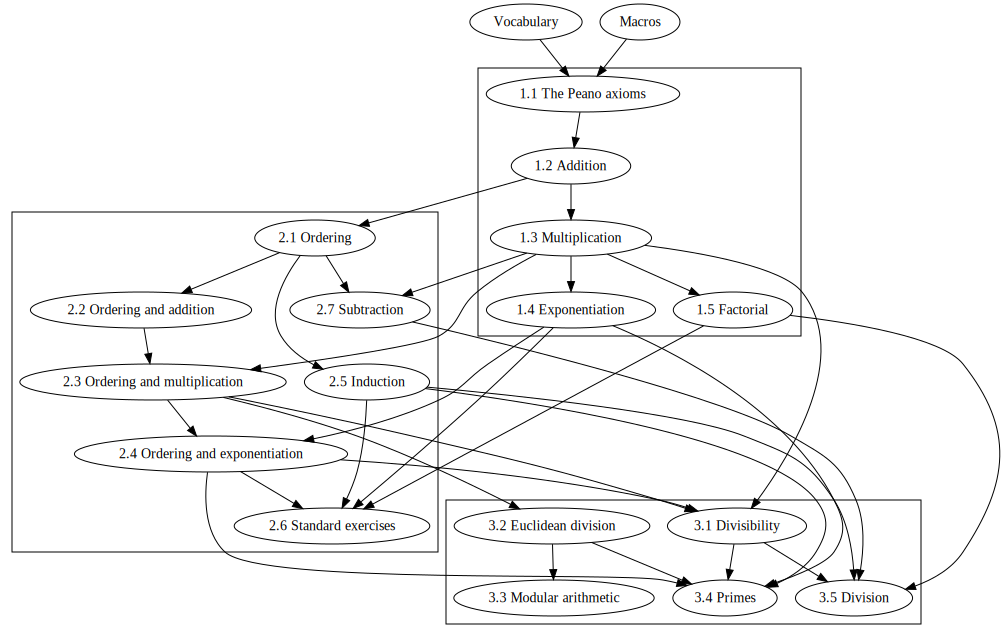
\includegraphics[width=0.9\linewidth]{./dependency-graph/graph.png}}
    \caption*{Interdependencies of the chapters}
  \end{figure}


  \section*{Introduction}

  This is a library providing a foundation of mathematics based on a
  Kelley-Morse like class theory with urelements.
  It introduces common operations on classes like unions or intersections
  (\cref{chapter:classes}) together with detailed proofs of their algebraic
  properties (\cref{chapter:computation-laws-for-classes}), the symmetric
  difference of two classes (\cref{chapter:symmetric-difference}) and the
  notions of ordered pairs and Cartesian products
  (\cref{chapter:pairs-and-products}) as well as proofs of the algebraic
  properties of the latter (\cref{chapter:computation-laws-for-products}).
  Moreover, it provides common operations on maps (\cref{chapter:maps}), various
  properties of images and preimages (\cref{chapter:image-and-preimage}) and the
  notions of injectivity, surjectivity, bijectivity
  (\cref{chapter:injections-surjections-bijections}) and invertibility of maps
  (\cref{chapter:invertible-maps}).
  The library provides an axiom system characterizing sets (\cref{chapter:sets})
  and, furthermore, it covers the notions of binary relations
  (\cref{chapter:binary-relations}), fixed-points of subset preserving maps
  (\cref{chapter:fixed-points}), including and equinumerosity
  (\cref{chapter:equinumerosity}).

  As two famous results it includes the Knaster-Tarski fixed point theorem
  (\cref{FOUNDATIONS_12_8420450166112256}) and the Cantor-Schröder-Bernstein
  theorem (\cref{FOUNDATIONS_13_1913663275401216}).

  \paragraph*{Usage.}
  At the very beginning of each chapter you can find the name of its source
  file, e.g. \path{foundations/sections/01_classes.ftl.tex} for
  \cref{chapter:classes}. This filename can be used to import the chapter via
  \Naproche's \texttt{readtex} instruction to another ForTheL text, e.g.:
  \begin{center}
    \verb`[readtex \path{foundations/sections/01_classes.ftl.tex}]`
  \end{center}

  \paragraph*{Checking times.}
  The checking times for each of the chapters may vary from computer to
  computer, but on mid-range hardware they are likely to be similar to those
  given in table below:

  \begin{center}
    \begin{tabular}{c|c|c}

      & \multicolumn{2}{c}{\textbf{Checking time}}
      \\
      \textbf{Chapter}
      & \textbf{without dependencies}     & \textbf{with dependencies}
      \\ \hline
      \ref{chapter:classes}
      & 00:04 min                         & 00:04 min
      \\
      \ref{chapter:computation-laws-for-classes}
      & 00:12 min                         & 00:16 min
      \\
      \ref{chapter:symmetric-difference}
      & 00:32 min                         & 00:48 min
      \\
      \ref{chapter:pairs-and-products}
      & 00:08 min                         & 00:12 min
      \\
      \ref{chapter:computation-laws-for-products}
      & 01:36 min                         & 01:56 min
      \\
      \ref{chapter:maps}
      & 01:13 min                         & 01:25 min
      \\
      \ref{chapter:image-and-preimage}
      & 01:28 min                         & 02:53 min
      \\
      \ref{chapter:injections-surjections-bijections}
      & 00:38 min                         & 02:03 min
      \\
      \ref{chapter:invertible-maps}
      & 02:20 min                         & 04:23 min
      \\
      \ref{chapter:sets}
      & 02:17 min                         & 06:40 min
      \\
      \ref{chapter:binary-relations}
      & 00:14 min                         & 06:54 min
      \\
      \ref{chapter:fixed-points}
      & 00:33 min                         & 07:13 min
      \\
      \ref{chapter:equinumerosity}
      & 01:48 min                         & 09:01 min
    \end{tabular}
  \end{center}


  \subfile{sections/01_classes.ftl.tex}
  \subfile{sections/02_computation-laws-for-classes.ftl.tex}
  \subfile{sections/03_symmetric-difference.ftl.tex}
  \subfile{sections/04_pairs-and-products.ftl.tex}
  \subfile{sections/05_computation-laws-for-products.ftl.tex}
  \subfile{sections/06_maps.ftl.tex}
  \subfile{sections/07_image-and-preimage.ftl.tex}
  \subfile{sections/08_injections-surjections-bijections.ftl.tex}
  \subfile{sections/09_invertible-maps.ftl.tex}
  \subfile{sections/10_sets.ftl.tex}
  \subfile{sections/11_binary-relations.ftl.tex}
  \subfile{sections/12_fixed-points.ftl.tex}
  \subfile{sections/13_equinumerosity.ftl.tex}
\end{document}

\documentclass[12pt,oneside]{book}

\usepackage[utf8]{inputenc}
\usepackage[english]{babel}

\usepackage{../meta-inf/lib/naproche-logo}
\usepackage{../meta-inf/lib/naproche}
\usepackage{../meta-inf/lib/libraries}
\usepackage{naproche}
\usepackage{naproche-libraries}
\renewcommand\libarchive{Preliminaries}
\usepackage{naproche}
\usepackage{naproche-libraries}
\renewcommand\libarchive{Preliminaries}

\usepackage{xr}
\externaldocument{../foundations/foundations}

\usepackage{graphicx}
\usepackage{float}
\usepackage{caption}
\usepackage[nobottomtitles]{titlesec}


\title{Set theory}
\author{Marcel Schütz}
\date{2022}

\begin{document}
  \maketitle

  \tableofcontents

  \paragraph*{}
  \begin{figure}[H]
    \centering
    \fbox{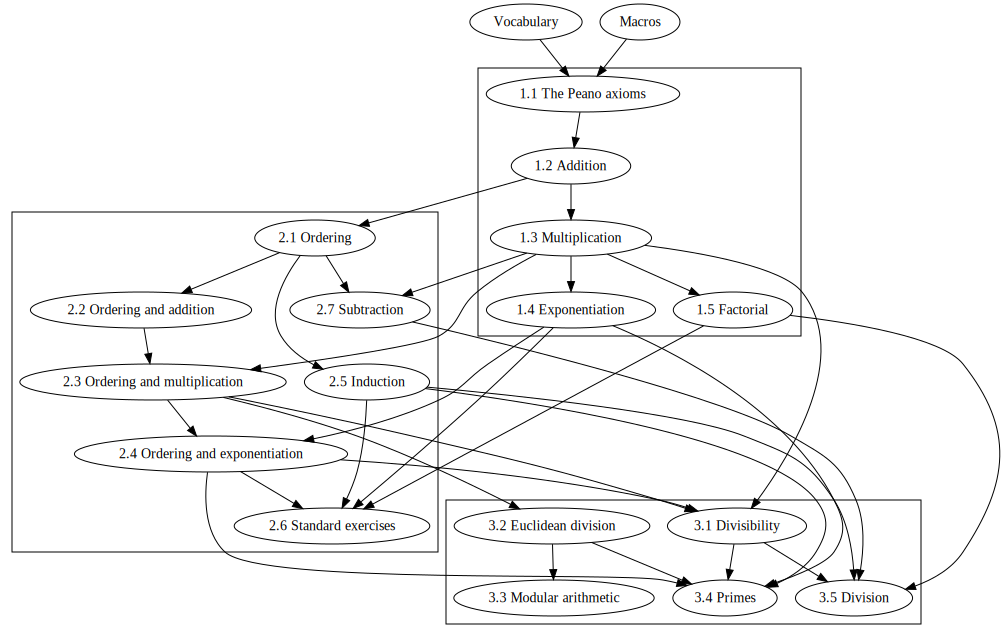
\includegraphics[width=0.9\textwidth]{./dependency-graph/graph.png}}
    \caption*{Interdependencies of the chapters}
  \end{figure}

  \section*{Introduction}

  This is a library providing basic results from undergraduate-level set theory.
  It introduces the notion of transitive classes
  (\cref{chapter:transitive-classes}), defines the notion of ordinal numbers
  (\cref{chapter:ordinals}) and as a special case of the latter introduces the
  set $\omega$ of finite ordinals (\cref{chapter:finite-ordinals}).
  Moreover, this library provides a formalization of the ordinal recursion
  theorem (\cref{chapter:recursion}) which is used to prove Zermelo's
  well-ordering theorem (\cref{chapter:zermelo}), on the basis of which the
  notion of cardinal numbers is introduced (\cref{chapter:cardinals}).
  Furthermore, some results about finite and infinite sets are given
  (\cref{chapter:finite-and-infinite-sets}).

  \paragraph*{Usage.}
  At the very beginning of each chapter you can find the name of its source
  file, e.g. \path{set-theory/sections/01_transitive-classes.ftl.tex} for
  \cref{chapter:transitive-classes}.
  This filename can be used to import the chapter via \Naproche's
  \texttt{readtex} instruction to another ForTheL text, e.g.:
  \begin{center}
    \verb`[readtex \path{set-theory/sections/01_transitive-classes.ftl.tex}]`
  \end{center}

  \paragraph*{Checking times.}
  The checking times for each of the chapters may vary from computer to
  computer, but on mid-range hardware they are likely to be similar to those
  given in table below:

  \begin{center}
    \begin{tabular}{c|c|c}

      & \multicolumn{2}{c}{\textbf{Checking time}}
      \\
      \textbf{Chapter}
      & \textbf{without dependencies}     & \textbf{with dependencies}
      \\ \hline
      \ref{chapter:transitive-classes}
      & 00:20 min                         & 07:00 min
      \\
      \ref{chapter:ordinals}
      & 03:20 min                         & 10:30 min
      \\
      \ref{chapter:finite-ordinals}
      & 01:15 min                         & 11:45 min
      \\
      \ref{chapter:recursion}
      & 04:05 min                         & 14:35 min
      \\
      \ref{chapter:zermelo}
      & 04:45 min                         & 21:40 min
      \\
      \ref{chapter:cardinals}
      & 05:10 min                         & 26:50 min
      \\
      \ref{chapter:finite-and-infinite-sets}
      & 10:50 min                         & 38:55 min
    \end{tabular}
  \end{center}

  \subfile{sections/01_transitive-classes.ftl.tex}
  \subfile{sections/02_ordinals.ftl.tex}
  \subfile{sections/03_finite-ordinals.ftl.tex}
  \subfile{sections/04_recursion.ftl.tex}
  \subfile{sections/05_well-ordering-theorem.ftl.tex}
  \subfile{sections/06_cardinals.ftl.tex}
  \subfile{sections/07_finite-and-infinite-sets.ftl.tex}
\end{document}

\begin{document}
  \begin{imports}
    \begin{forthel}
      %[prove off][check off]
      [readtex \path{libraries/source/set-theory/zero.ftl.tex}]
      [readtex \path{libraries/source/set-theory/successor-ordinals.ftl.tex}]
      %[prove on][check on]
    \end{forthel}
  \end{imports}


  \section*{Natural Numbers}

  \begin{forthel}
    \begin{definition}[id=SET_THEORY_03_4310076227584000,printid]
      \[ \omega = \class{n \in \Ord | \classtext{$n \in X$ for every $X \subseteq \Ord$ such that $0 \in X$ and for all $x \in X$ we have $\succ(x) \in X$}}. \]
    \end{definition}

    Let a natural number stand for an element of $\omega$.
  \end{forthel}

  \begin{forthel}
    \begin{proposition}[id=SET_THEORY_03_3576717620805632,printid]
      $0 \in \omega$.
    \end{proposition}
  \end{forthel}

  \begin{forthel}
    \begin{proposition}[id=SET_THEORY_03_8807317141192704,printid]
      Let $n \in \omega$.
      Then $\succ(n) \in \omega$.
    \end{proposition}
  \end{forthel}

  \begin{forthel}
    \begin{proposition}[id=SET_THEORY_03_344585425387520,printid]
      Let $\Phi \subseteq \omega$.
      Assume that $0 \in \Phi$ and for every $x \in \Phi$ we have
      $\succ(x) \in \Phi$.
      Then $\Phi = \omega$.
    \end{proposition}
    \begin{proof}
      Suppose $\Phi \neq \omega$.
      Consider an element $n$ of $\omega$ that is not contained in $\Phi$.
      Take $\Phi' = \Phi \setminus \set{n}$.

      (1) $0 \in \Phi'$.
      Indeed $0 \in \Phi$ and $0 \neq n$.

      (2) For each $x \in \Phi'$ we have $\succ(x) \in \Phi'$. \\
      Proof.
        Let $x \in \Phi'$.
        Then $\succ(x) \in \Phi$.

        Let us show that $\succ(x) \neq n$.
          Assume $\succ(x) = n$.
          Then $x \notin \Phi$.
          Indeed $n \notin \Phi$ and if $x \in \Phi$ then
          $n = \succ(x) \in \Phi$.
          Contradiction.
        End.

        Thus $\succ(x) \in \Phi'$.
      Qed.

      Therefore every element of $\omega$ lies in $\Phi'$.
      Indeed $\Phi' \subseteq \Ord$.
      Consequently $n \in \Phi'$.
      Contradiction.
    \end{proof}
  \end{forthel}

  \begin{forthel}
    \begin{corollary}[id=SET_THEORY_03_4847727433220096,printid]
      $\omega$ is a set.
    \end{corollary}
    \begin{proof}
      Define $f(n) = \succ(n)$ for $n \in \omega$.
      Take a subset $X$ of $\omega$ that is inductive regarding $0$ and $f$.
      Indeed $f$ is a map from $\omega$ to $\omega$.
      Then we have $0 \in X$ and for each $n \in X$ we have $\succ(n) \in X$.
      Thus $X = \omega$.
      Therefore $\omega$ is a set.
    \end{proof}
  \end{forthel}

  \begin{forthel}
    \begin{proposition}[id=SET_THEORY_03_5885789275684864,printid]
      Let $n \in \omega$.
      Then $n = 0$ or $n = \succ(m)$ for some $m \in \omega$.
    \end{proposition}
    \begin{proof}
      Assume the contrary.
      Consider a $k \in \omega$ such that neither $k = 0$ nor $k = \succ(m)$ for
      some $m \in \omega$.
      Take a class $\omega'$ such that $\omega' = \omega \setminus \set{k}$. %!
      Then $\omega'$ is a set.

      (1) $0 \in \omega'$.
      Indeed $k \neq 0$.

      (2) For all $m \in \omega'$ we have $\succ(m) \in \omega'$. \\
      Proof.
        Let $m \in \omega'$.
        Then $\succ(m) \neq k$.
        Hence $\succ(m) \in \omega'$.
      Qed.

      Thus every element of $\omega$ is contained in $\omega'$.
      Therefore $k \in \omega'$.
      Contradiction.
    \end{proof}
  \end{forthel}

  \begin{forthel}
    \begin{proposition}[id=SET_THEORY_03_5057540872208384,printid]
      Every element of $\omega$ is an ordinal.
    \end{proposition}
  \end{forthel}
\end{document}
